\chapter{Wazuh \acrshort{gui}}
\section{Startseite}
Die Wazuh Startseite kann mit dem Webbrowser aufgerufen werden.\\

Auf der Startseite sieht man alle aktiven und inaktiven Computer, die mit dem Wazuh Manager verbunden sind.
Von hier aus hat man Schnellzugriff auf alle ``Module'', die Wazuh anbietet.\\

Alle Module und Einstellungen findet man auch im Menü, welches sich durch klicken vom Wazuh Logo öffnen lässt.
\begin{figure}[H]
    \centering
    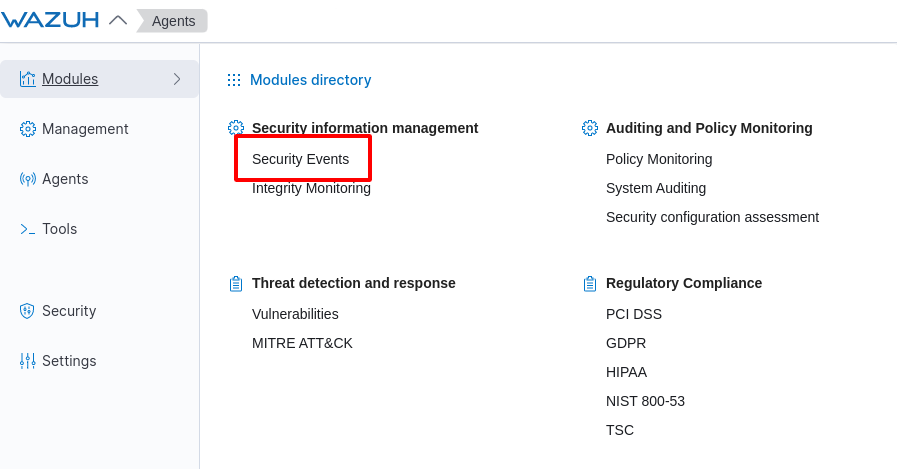
\includegraphics[width=\linewidth]{../img/wazuh-menu.png}
    \caption{Wazuh Menü}
\end{figure}

\section{Security Events}
Die Security Events findet man unter \textbf{Wazuh $\rightarrow$ Modules $\rightarrow$ Security Events}.
Im Modul Security Events werden alle Alerts angezeigt, welche durch die definierten Regeln ausgelöst werden.

\begin{figure}[H]
    \centering
    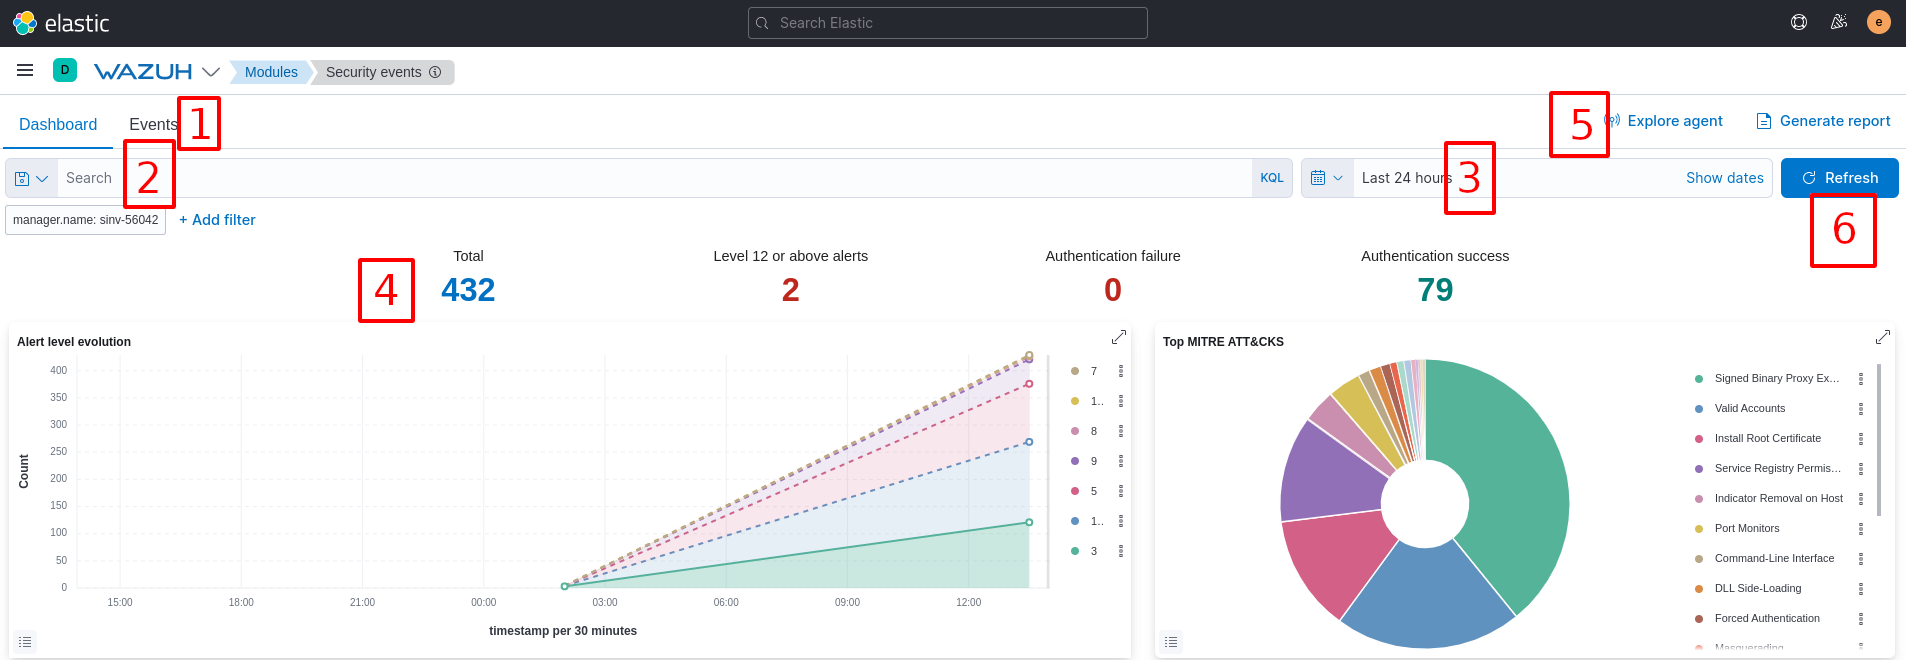
\includegraphics[width=\linewidth]{../img/wazuh-se-1.png}
    \caption{Security Events}
\end{figure}
\begin{enumerate}
    \item Navigation zwischen dem Dashboard und den Events. Das Dashboard zeigt die Alerts und zusammenfassende Diagramme an. Unter Events sieht man nur die Alerts, dafür aber zusätzlich bessere Filter.
    \item In diesem Eingabefeld kann man die Alerts durchsuchen. Mithilfe von Filtern kann man gewünschte Alerts ausblenden oder nur gewählte Anzeigen lassen.
    \item Hier kann man die Zeitspanne angeben, wie lange zurück man die Alerts ansehen möchte.
    \item Diese Übersicht zeigt an, wie viele Alerts in der eingestellten Zeitspanne generiert wurden und wieviele davon über Level 12 (Kritisch) sind, wieviele davon erfolgreiche Logins und wieviele fehlgeschlagene Logins. Ausserdem zeigt es noch zusammenfassende Diagramme an.
    \item Bei ``Explore Agent'' kann man einen Agent auswählen um nur dessen Alerts anzuzeigen.
    \item Mit ``Refresh'' kann man die neusten Alerts laden.
\end{enumerate}

Auf der Seite unten findet man auch die Alerts. 
In der Liste werden die Alerts angeziegt. 
Diese können nach Titel sortiert werden. 
\begin{figure}[H]
    \centering
    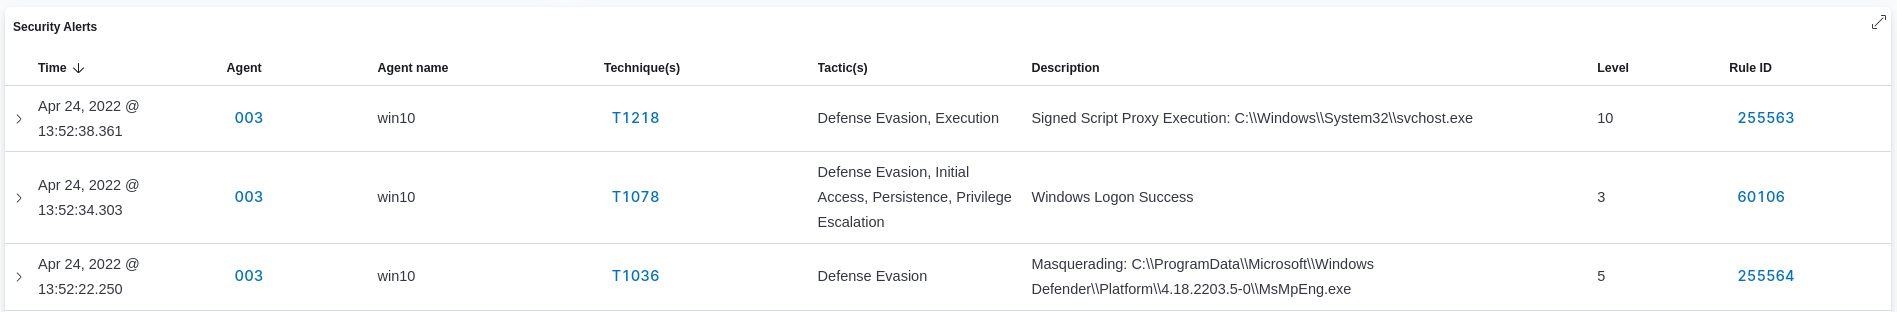
\includegraphics[width=\linewidth]{../img/wazuh-se-2.png}
    \caption{Security Events}
\end{figure}


\begin{itemize}
    \item \textbf{Time} zeigt die Zeit, wann der Alert eingegenen ist.
    \item \textbf{Agent} zeigt von welchem Agent der Alert eingegenen ist.
    \item \textbf{Agent name} zeigt den Hostname des Agent.
    \item \textbf{Technique \& Tatic} zeigt die \href{https://attack.mitre.org/techniques/enterprise/}{Mitre Attack Framework}\footnote{Link: \href{https://attack.mitre.org/techniques/enterprise/}{https://attack.mitre.org/techniques/enterprise/}} Technik an, welcher dieser Alert sein könnte.
    \item \textbf{Description} zeigt eine Beschreibung, um was es sich bei diesem Alert handelt.
    \item \textbf{Level} zeigt das Level des Alerts an. 
    \item \textbf{Rule ID} zeigt an, welche Regel diesen Alert generiert hat.
\end{itemize}

\section{Integrity Monitoring}
Das Integrity Monitoring findet man unter \textbf{Wazuh $\rightarrow$ Modules $\rightarrow$ Integrity Monitoring}.
Im Inventory Monitoring werden alle veränderten Systemdateien und Registry Einträge geloggt. 
Damit kann man bei einem Sicherheitsvorfall eventuell nachvollziehen, wie vorgegangen wurde.

\begin{figure}[H]
    \centering
    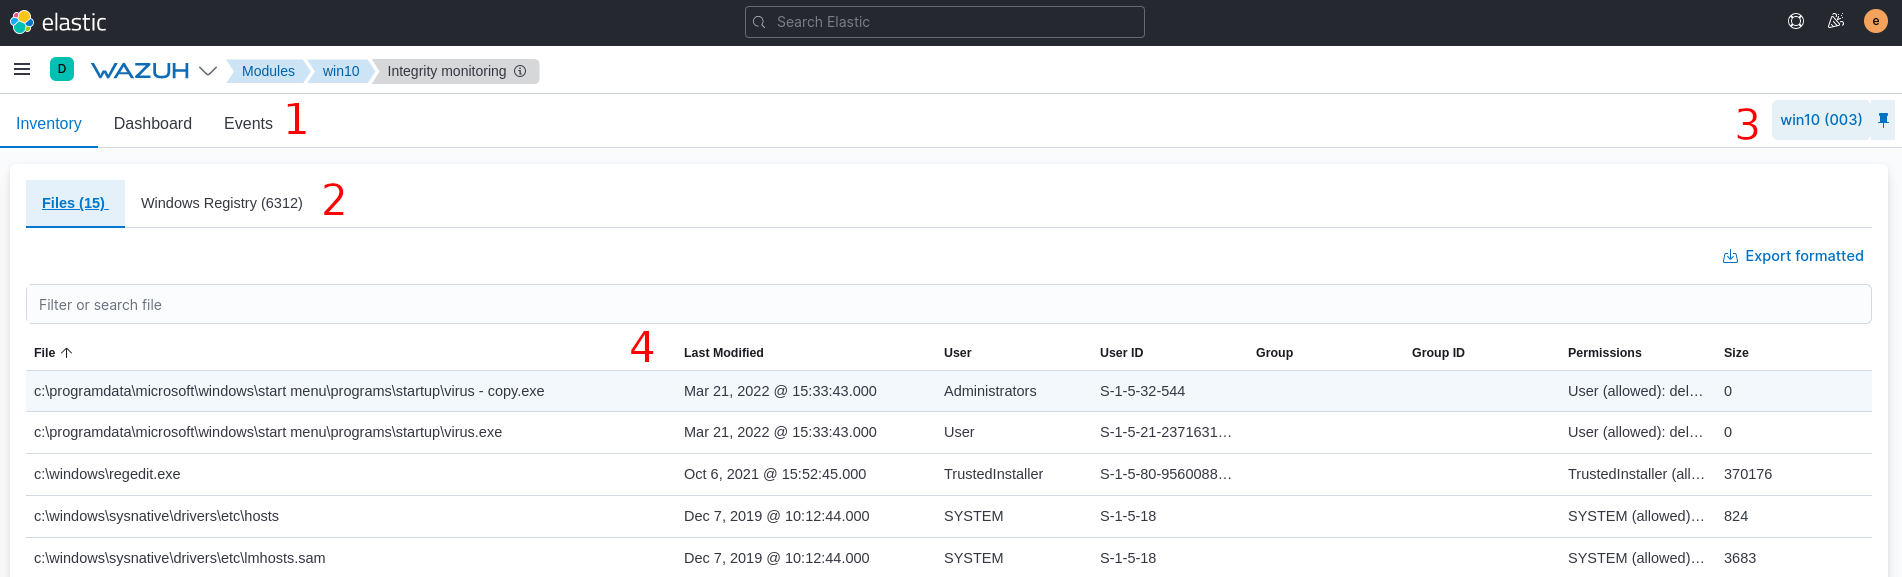
\includegraphics[width=\linewidth]{../img/wazuh-im-inventory.png}
    \caption{Inventory Monitoring}
\end{figure}

\begin{enumerate}
    \item Navigation zwischen dem Inventory, dem Dashboard und den Events.
    \textbf{Inventory} zeigt die veränderten Systemdateien und Registry Einträge an. Im \textbf{Dashboard} findet man zusammenfassende Diagramme und unter \textbf{Events} werden auch alle Änderungen angezeigt, aber zusätzlichen mit einer unterstützenden Suche. 
    \item Navigation zwischen den geänderten Systemdateien und Registry Einträgen.
    \item Agent auswählen, welcher man anschauen möchte.
    \item Liste von bearbeiteten Systemdateien oder Registry Einträgen.
\end{enumerate}

\section{Rules}
Die Regeln findet man unter \textbf{Wazuh $\rightarrow$ Management $\rightarrow$ Rules}.
Hier können alle Regeln angeschaut und eigene Regeln hinzugefügt werden. 

\begin{figure}[H]
    \centering
    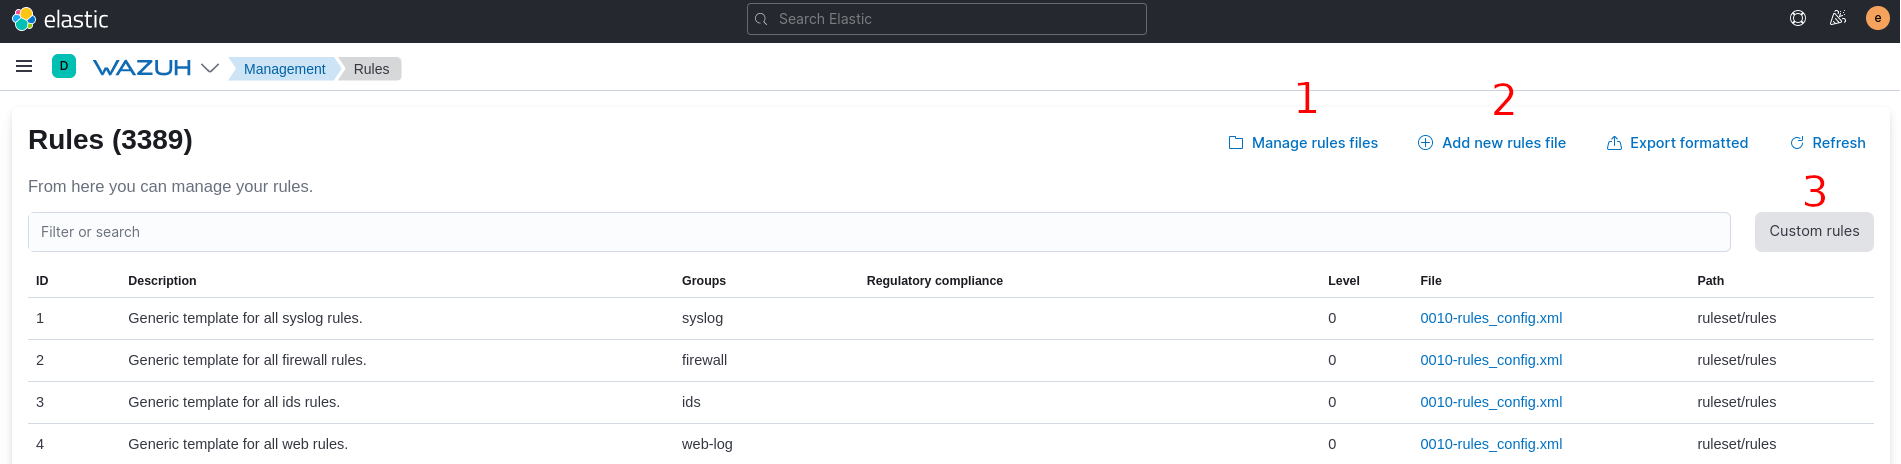
\includegraphics[width=\linewidth]{../img/wazuh-rules.png}
    \caption{Rules}
\end{figure}

\begin{enumerate}
    \item ``Manage rules files'' kann alle Dateien, welche die Regeln beinhalten, anschauen. 
    \item ``Add new rules file'' kann eine neue Datei hinzufügen, um neue Regeln zu definieren.
    \item ``Custom rules'' kann die eigenen Regeln oder Regeldateien anzeigen lassen. Alle Regeln von Wazuh werden ausgeblendet.
\end{enumerate}

\section{Decoders}
Das Decoder findet man unter \textbf{Wazuh $\rightarrow$ Management $\rightarrow$ Decoders}.
Diese Seite ist gleich aufgebaut wie die Rules Seite.

\section{Groups}
Die Gruppen findet man unter \textbf{Wazuh $\rightarrow$ Management $\rightarrow$ Groups}.
Auf dieser Seite findet man alle definierten Gruppen, kann neue Gruppen hinzufügen und entfernen.

\begin{figure}[H]
    \centering
    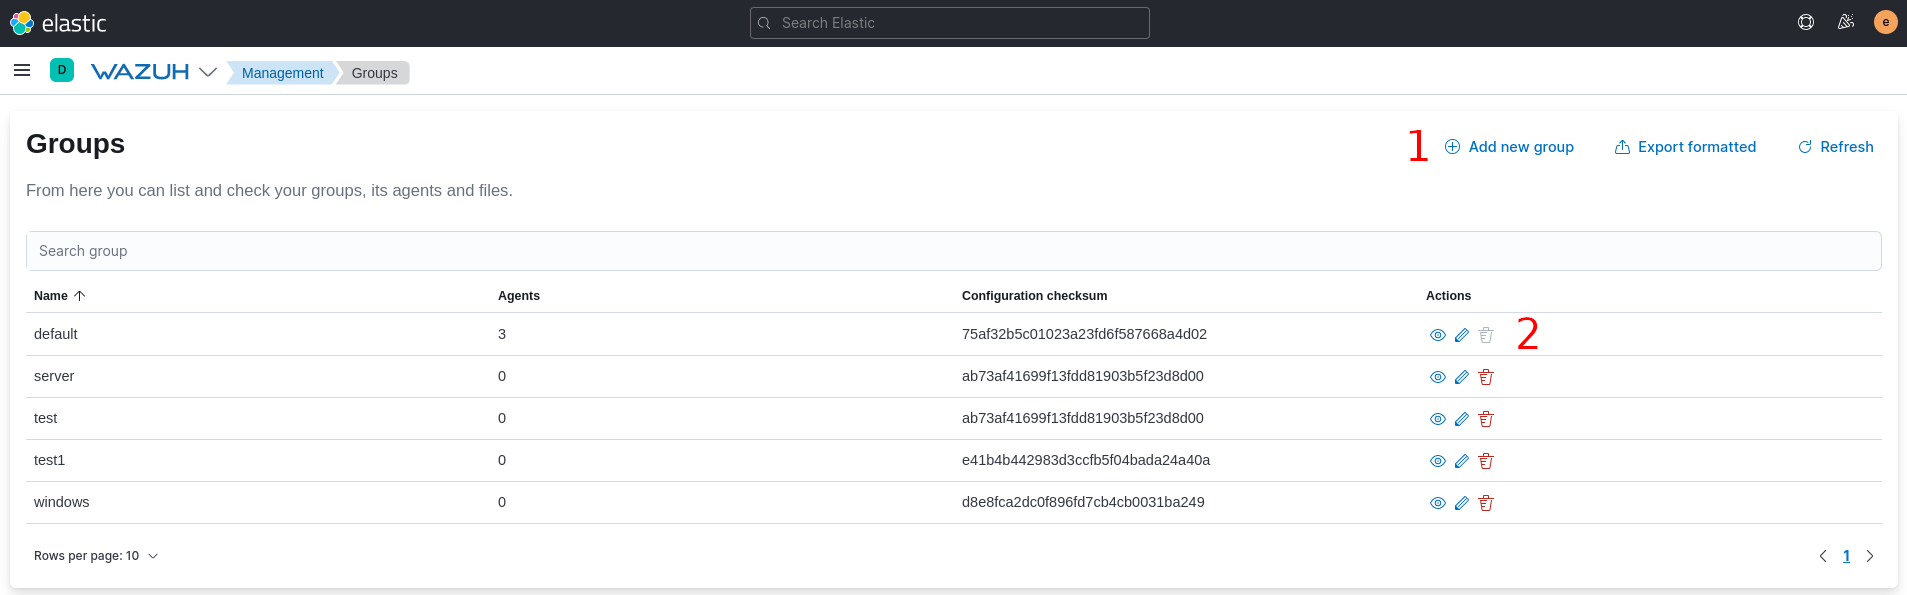
\includegraphics[width=\linewidth]{../img/wazuh-groups.png}
    \caption{Groups}
\end{figure}

\begin{enumerate}
    \item ``Add new group'' kann eine neue Gruppe hinzufügen.
    \item Hier kann man die einzelnen Gruppen verwalten. Mit dem Aug-Symbol kann man alle Agents anschauen, die dieser Gruppe zugewiesen sind. Mit dem Stift-Symbol kann man die agent.conf bearbeiten und mit dem Papierkorb-Symbol kann man die Gruppe löschen. 
\end{enumerate}

\section{Konfiguration des Managers}
Die Konfiguration findet man unter \textbf{Wazuh $\rightarrow$ Management $\rightarrow$ Configuration}.
Hier gibt es eine Übersicht von allen Wazuh Manager Einstellungen und diese können bearbeitet werden.

\section{Wazuh Agents}
Die Konfiguration findet man unter \textbf{Wazuh $\rightarrow$ Agents}.
Hier sieht man alle registrierten Agents und kann neue Agents hinzufügen.

\begin{figure}[H]
    \centering
    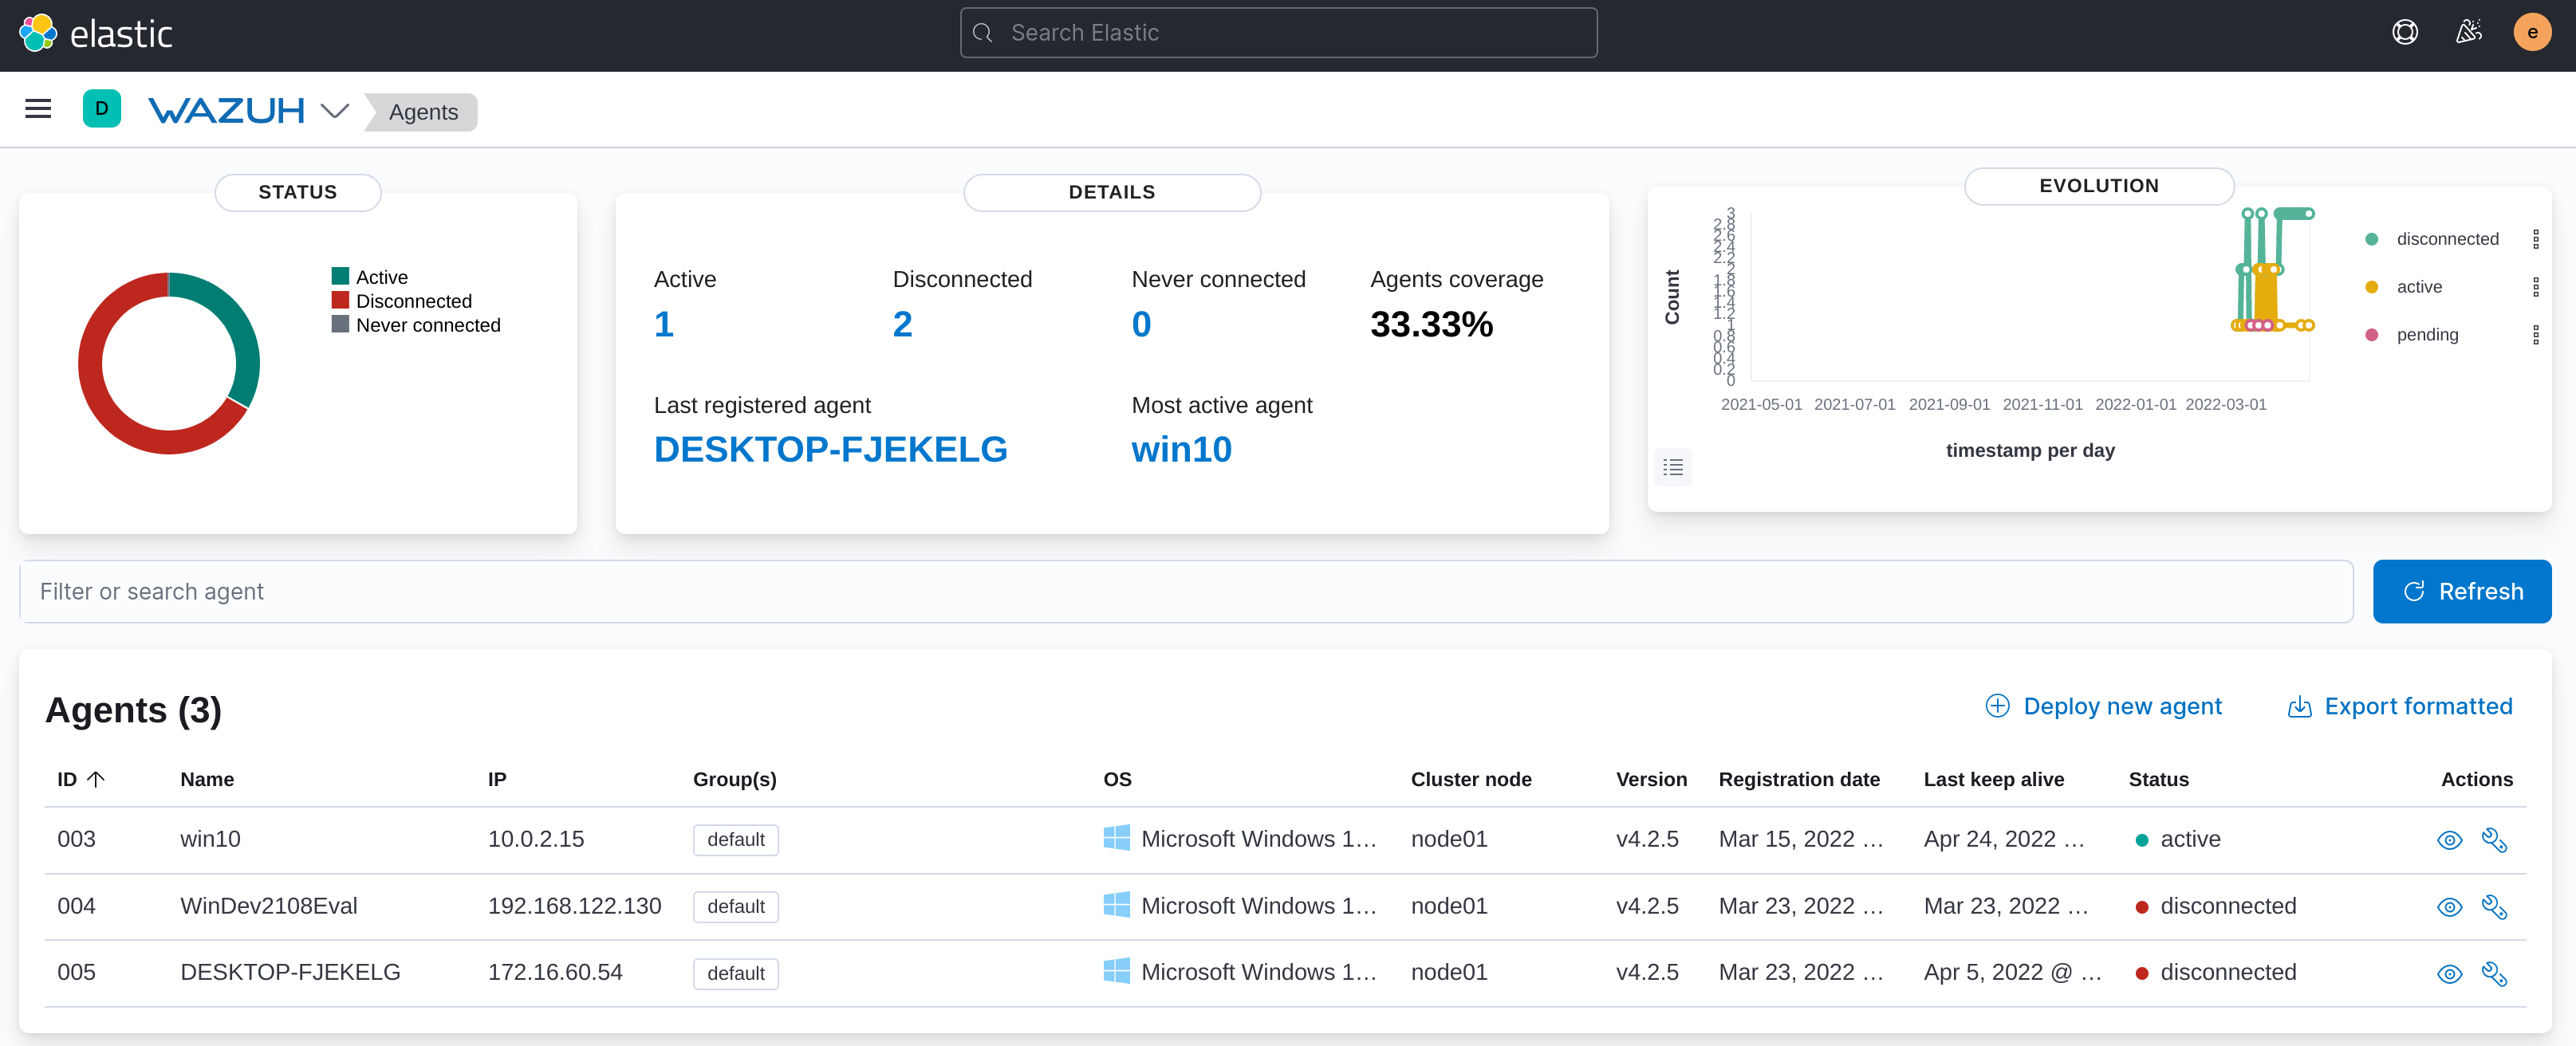
\includegraphics[width=\linewidth]{../img/wazuh-agents.png}
    \caption{Agents}
\end{figure}

